\begin{frame}[label=results]{Structure: Results}
    \frametitle{Structure}
    \begin{itemize}
        \item Research Questions
        \item Background \& Literature
        \item {\color{tud grapefruit}Preliminary Results}
        \item Outlook
    \end{itemize}
\end{frame}

\footerinfootnotesfalse
\begin{frame}[label=results,fragile]{Results: Multi-cluster}
    \frametitle{Preliminary Results}
    \framesubtitle{Generalization to multiple clusters}
    \only<1-2>{%
        \begin{figure}
            \centering
            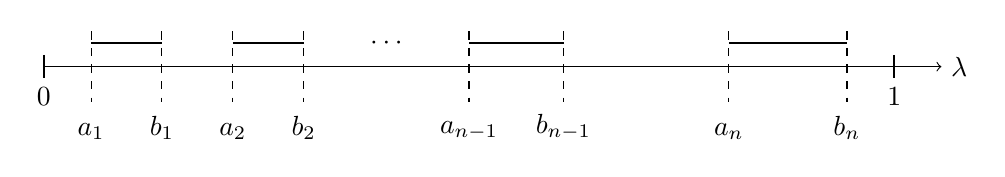
\begin{tikzpicture}[scale=3]

    % Axis
    \draw[->] (0,0) -- (3.8,0) node[right] {$\lambda$};

    % Tick marks and labels at 0 and 1
    \foreach \x/\label in {0/0, 3.6/1}
    {
        \draw[thick] (\x,0.05) -- (\x,-0.05);
        \node[below=4pt] at (\x,0) {$\label$};
    }

    % Multiple disjoint clusters
    \draw[thick] (0.2,0.1) -- (0.5,0.1); % Cluster 1
    \draw[thick] (0.8,0.1) -- (1.1,0.1); % Cluster 2
    \draw[thick] (1.8,0.1) -- (2.2,0.1); % Cluster 3
    \draw[thick] (2.9,0.1) -- (3.4,0.1); % Cluster 4

    % Dots indicating missing middle clusters
    \node at (1.45,0.1) {$\cdots$};

    % Mark points a_1, b_1, a_2, b_2, ..., a_n, b_n
    \foreach \x/\label in {
        0.2/{a_1}, 0.5/{b_1},
        0.8/{a_2}, 1.1/{b_2},
        1.8/{a_{n-1}}, 2.2/{b_{n-1}},
        2.9/{a_n}, 3.4/{b_n}
    }
    {
        \draw[thin,dashed] (\x,0.15) -- (\x,-0.15);
        \node[above] at (\x,-0.35) {$\label$};
    }

\end{tikzpicture}
        \end{figure}
    }
    \only<2>{%
        Building on the work of \citeauthor{cg_sharpened_convrate_Axelsson1976} we can imagine $r_{\bar{m}} = \hat{r}_{p_1}\hat{r}_{p_2}\dots\hat{r}_{p_n}\in\mathcal{P}_{\bar{m}}$ with
        \begin{equation*}
            p_i \leq \left\lceil\log_{f_i}{\frac{\epsilon}{2}} + \sum_{j=1}^{i-1} p_j\log_{f_i}{\frac{\zeta^{(j)}_2}{\zeta^{(i,j)}_1}} \right\rceil \quad \text{and} \quad f_i =\frac{\sqrt{\kappa_i}-1}{\sqrt{\kappa_i}+1}.
        \end{equation*}
        Sharpened bound given by
        \begin{equation*}
            \bar{m} = \sum_{i=1}^{n} p_i.
        \end{equation*}
    }
    \only<3>{%
        \begin{figure}
            \centering
            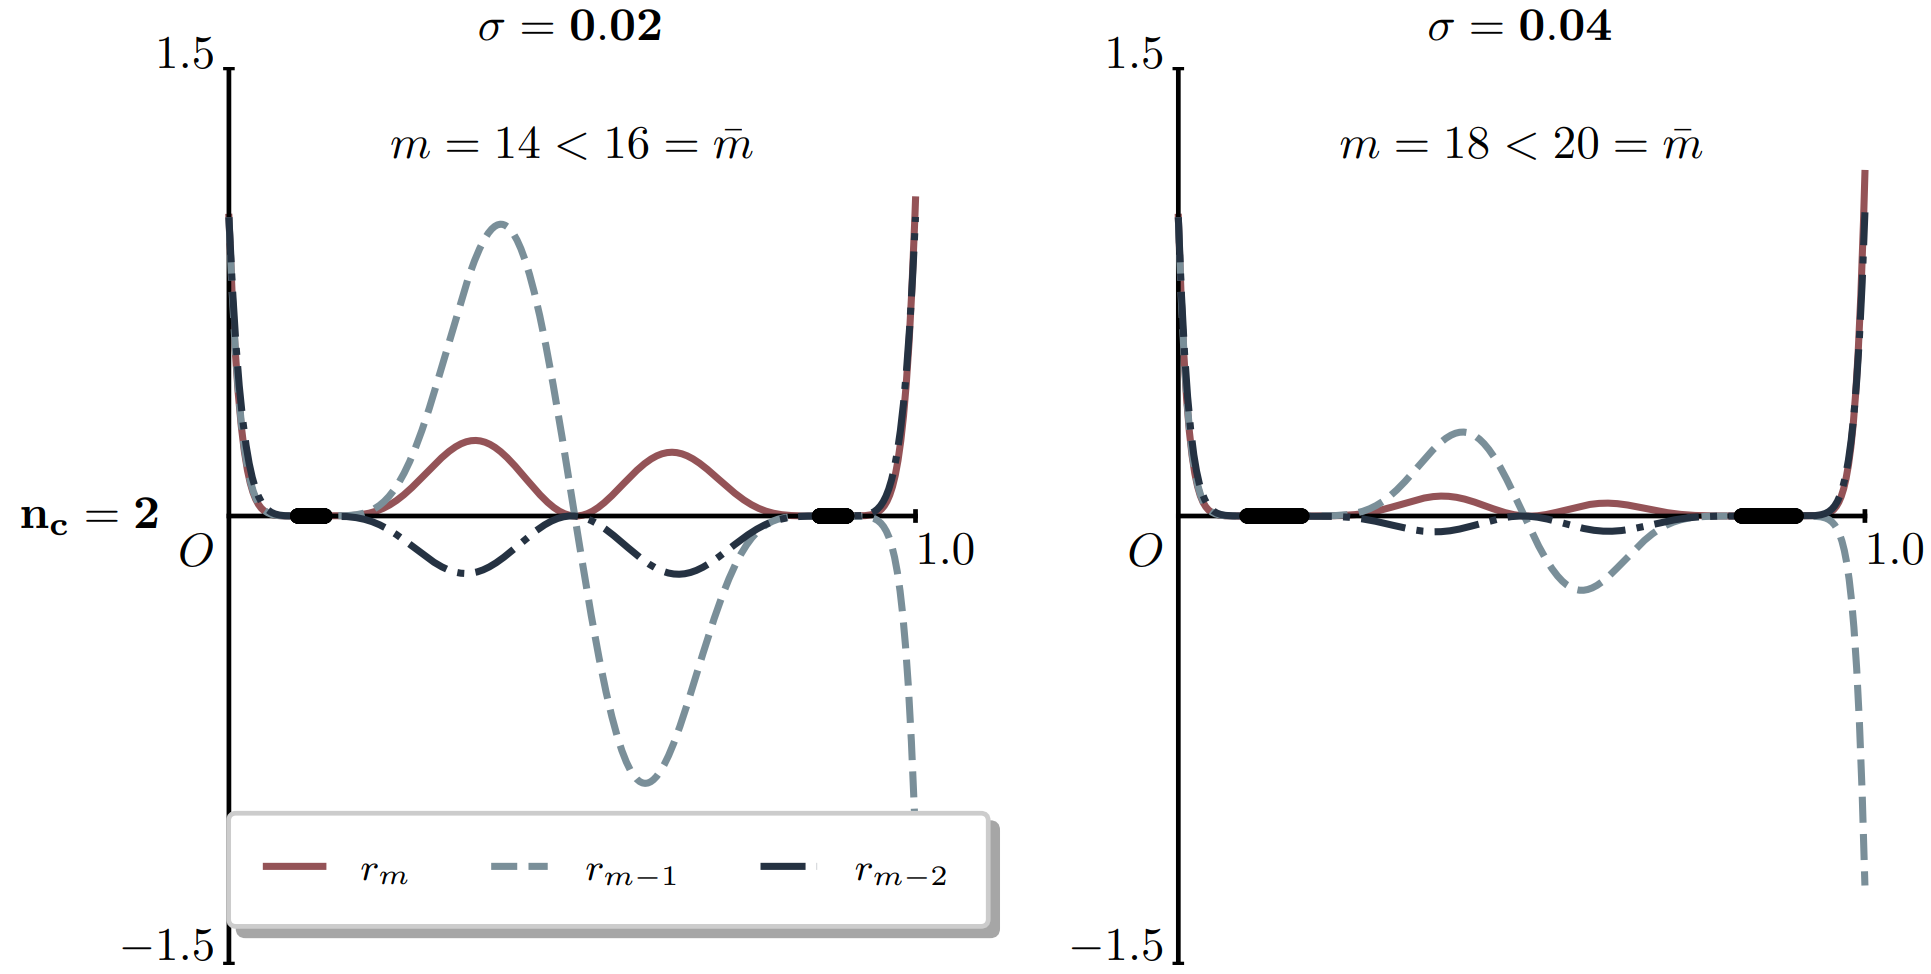
\includegraphics[width=0.8\textwidth]{sharpened_bound_2_clusters.png}
        \end{figure}
    }
    \only<4>{%
        \begin{figure}
            \centering
            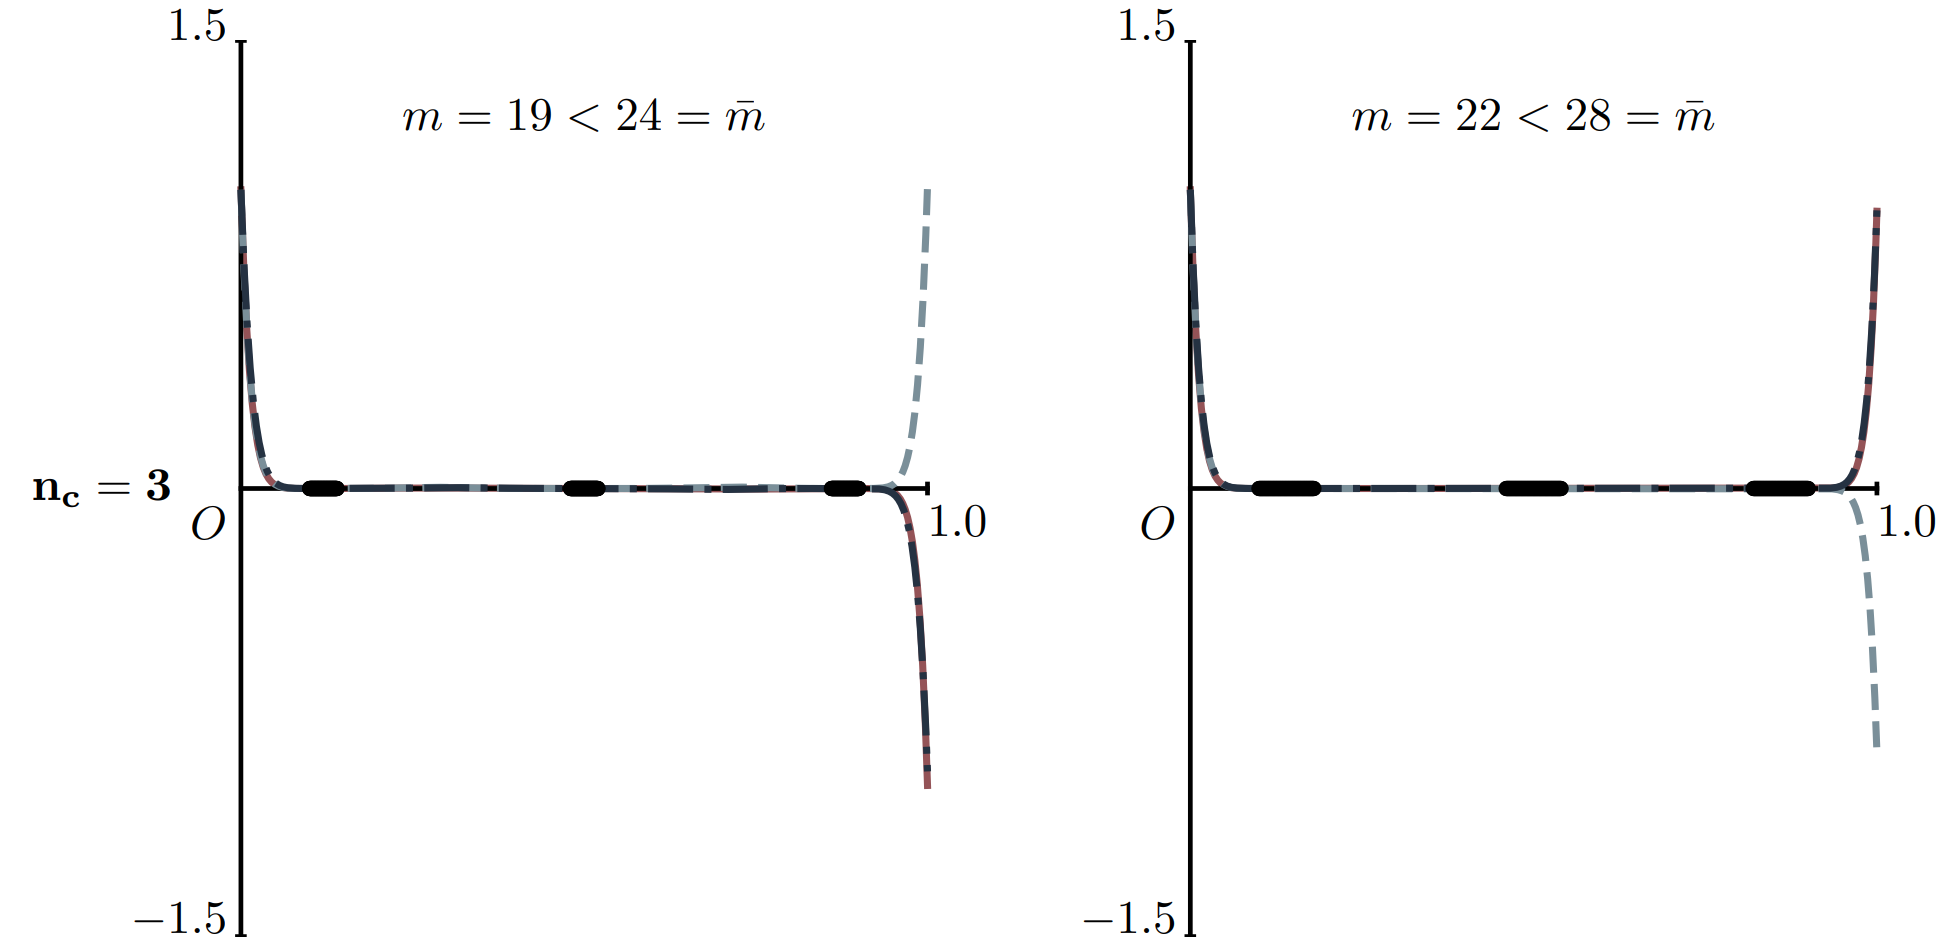
\includegraphics[width=0.8\textwidth]{sharpened_bound_3_clusters.png}
        \end{figure}
    }
\end{frame}

\begin{frame}[label=results,fragile]{Results: Demo}
    \frametitle{Preliminary Results}
    \framesubtitle{Demo}
\end{frame}